\subsection{Data}
The PAD-UFES-20 data set contains 26 columns and 2,299 rows which adds up to a total of 59,748 entries not including the column names. There are a total of 10,484 missing values which represent the 17.54\% of all entries.
\newline
It is worth to note that out of the 26 columns, 11 have exactly 804 missing values, which suggests that 804 lesions don’t have most of the background information.
\newline
We can count 1,641 unique lesion IDs, but only 1,373 unique patient IDs, so we can conclude that some patients have multiple lesions registered. Likewise there must also be multiple pictures of the same lesions.

\subsection{Approach}
The report follows a step by step structure to classify the images into melanoma and non-melanoma.

\subsubsection{Annotations and Feature Extraction}
Before writing our own annotation guide, we reviewed the slides and reference materials from our lectures in Projects in Data Science. This allowed us to write guidelines for systematically annotating asymmetry, colour variation, and the presence of blue-white veil in skin lesions.
\newline
Asymmetry is rated on a scale from 1 to 3, where a score of 1 indicates that the lesion is clearly symmetric, 2 suggests partial symmetry, and 3 denotes a complete lack of symmetry.
\newline
Colour variation is also rated from 1 to 3, with 1 representing even colouration, 2 indicating some variation, and 3 suggesting significant variation.
\newline
For blue-white veil, the scores are binary with 0 meaning that the veil is not present, and 1 that it is.

\begin{figure}[H]
    \centering
    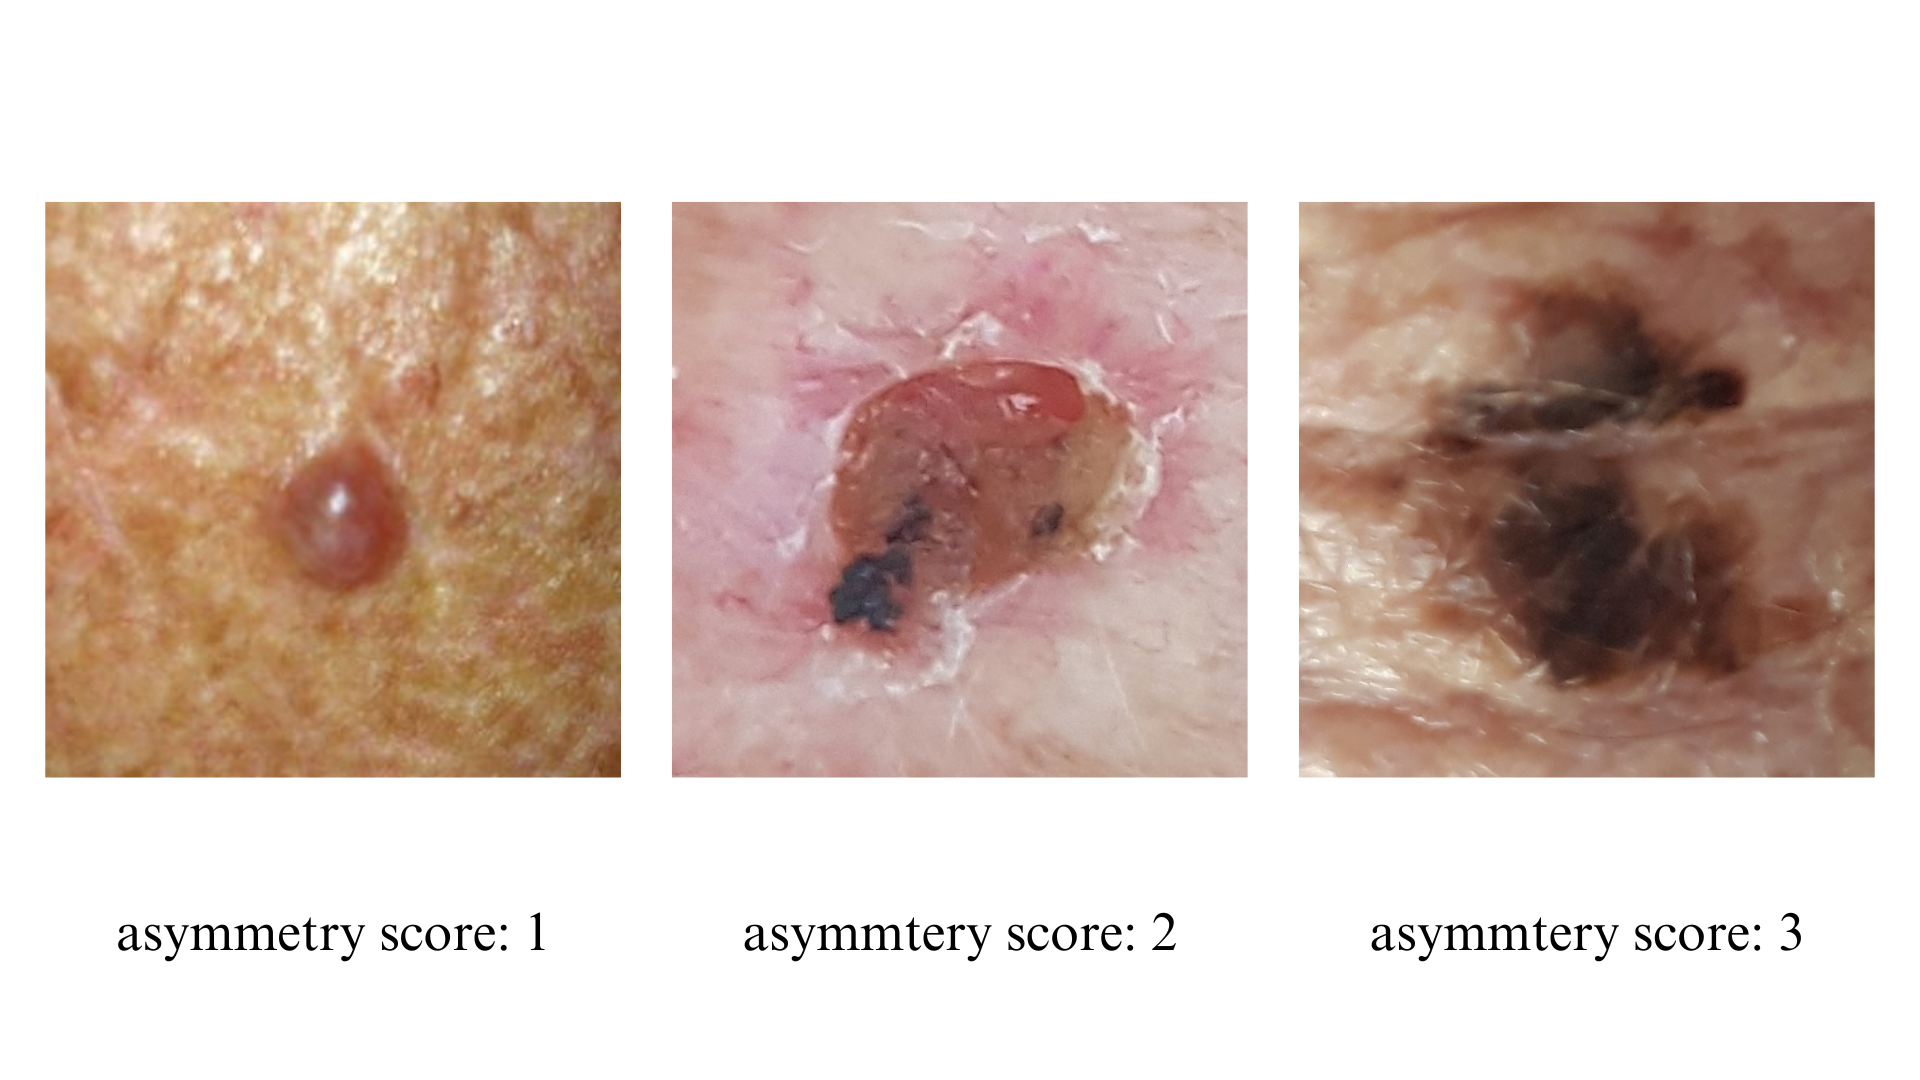
\includegraphics[width=1\linewidth]{asymmetryy.png}
    \caption{Asymmetry score}
    \label{fig:Asymmetry score}
\end{figure}

\begin{figure}[H]
    \centering
    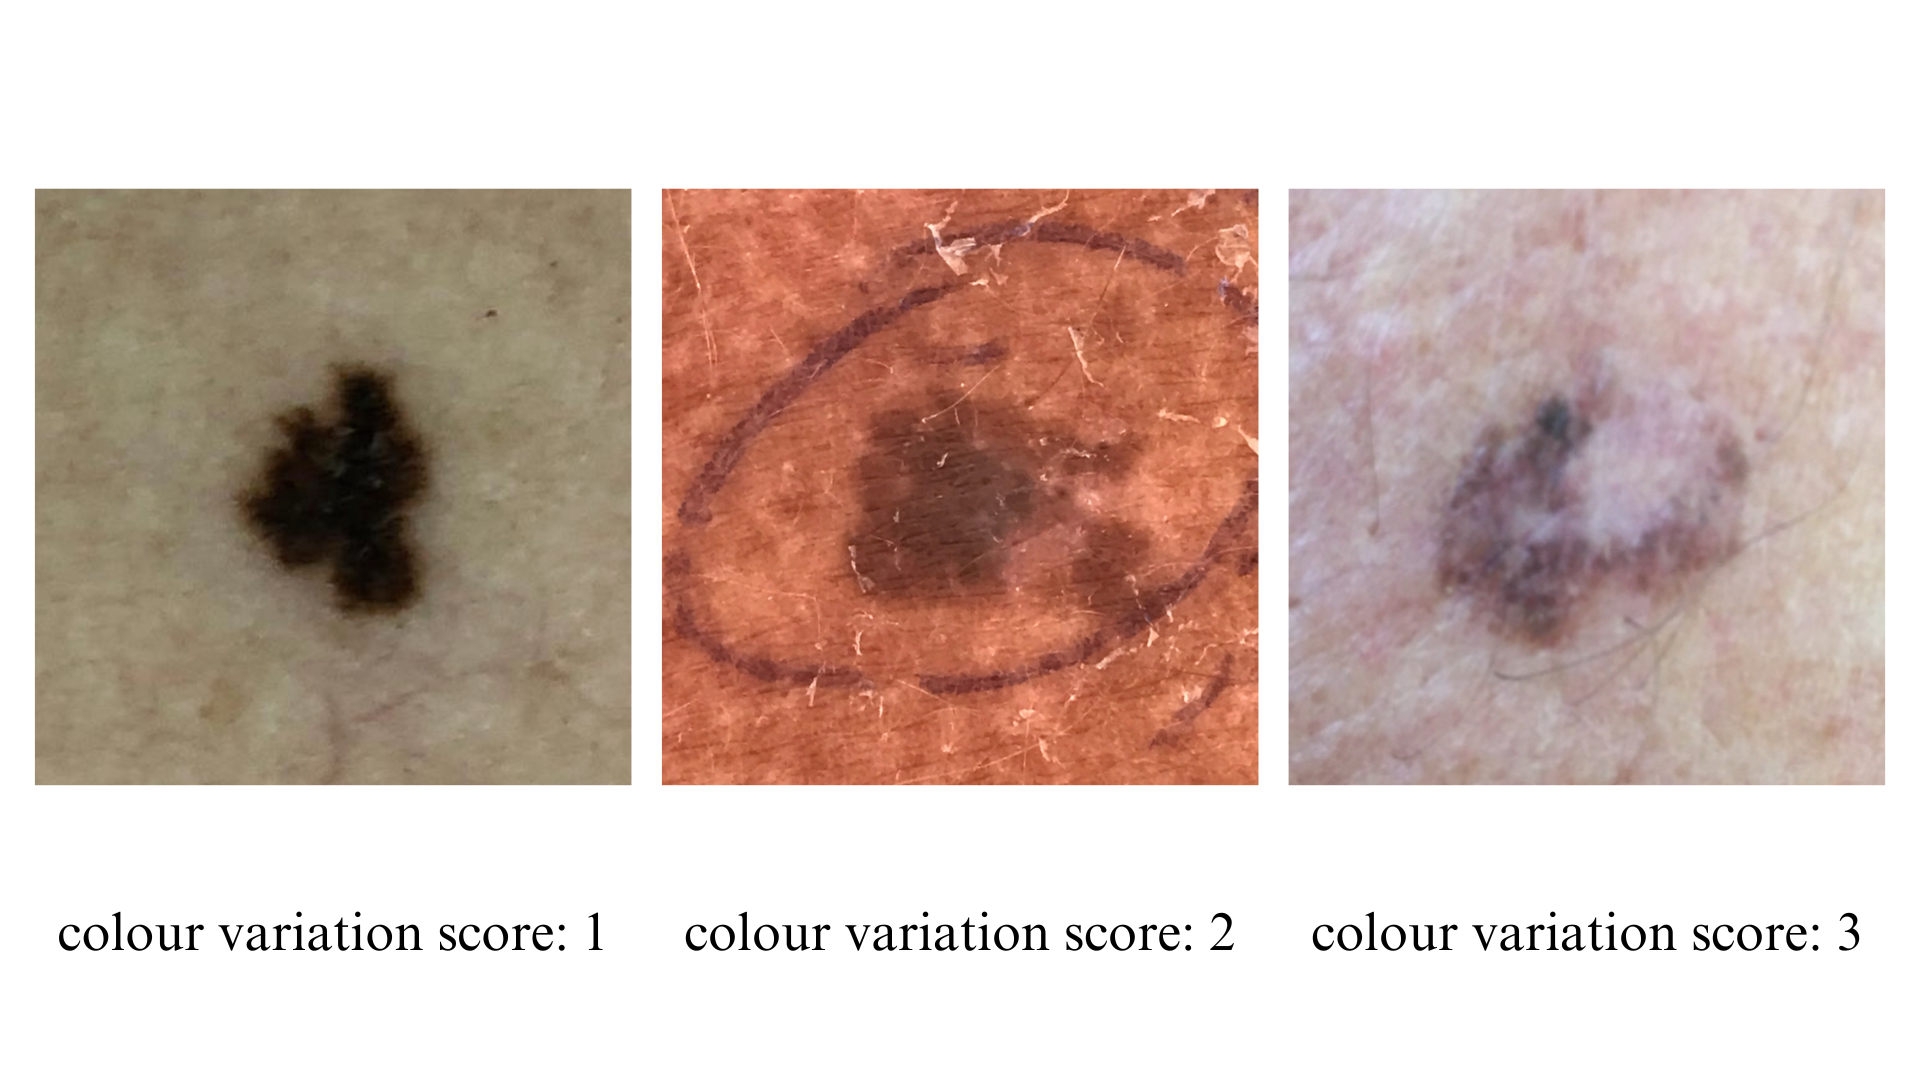
\includegraphics[width=1\linewidth]{colour variation.png}
    \caption{Colour variation score}
    \label{fig:Colour variation score}
\end{figure}

\begin{figure}[H]
    \centering
    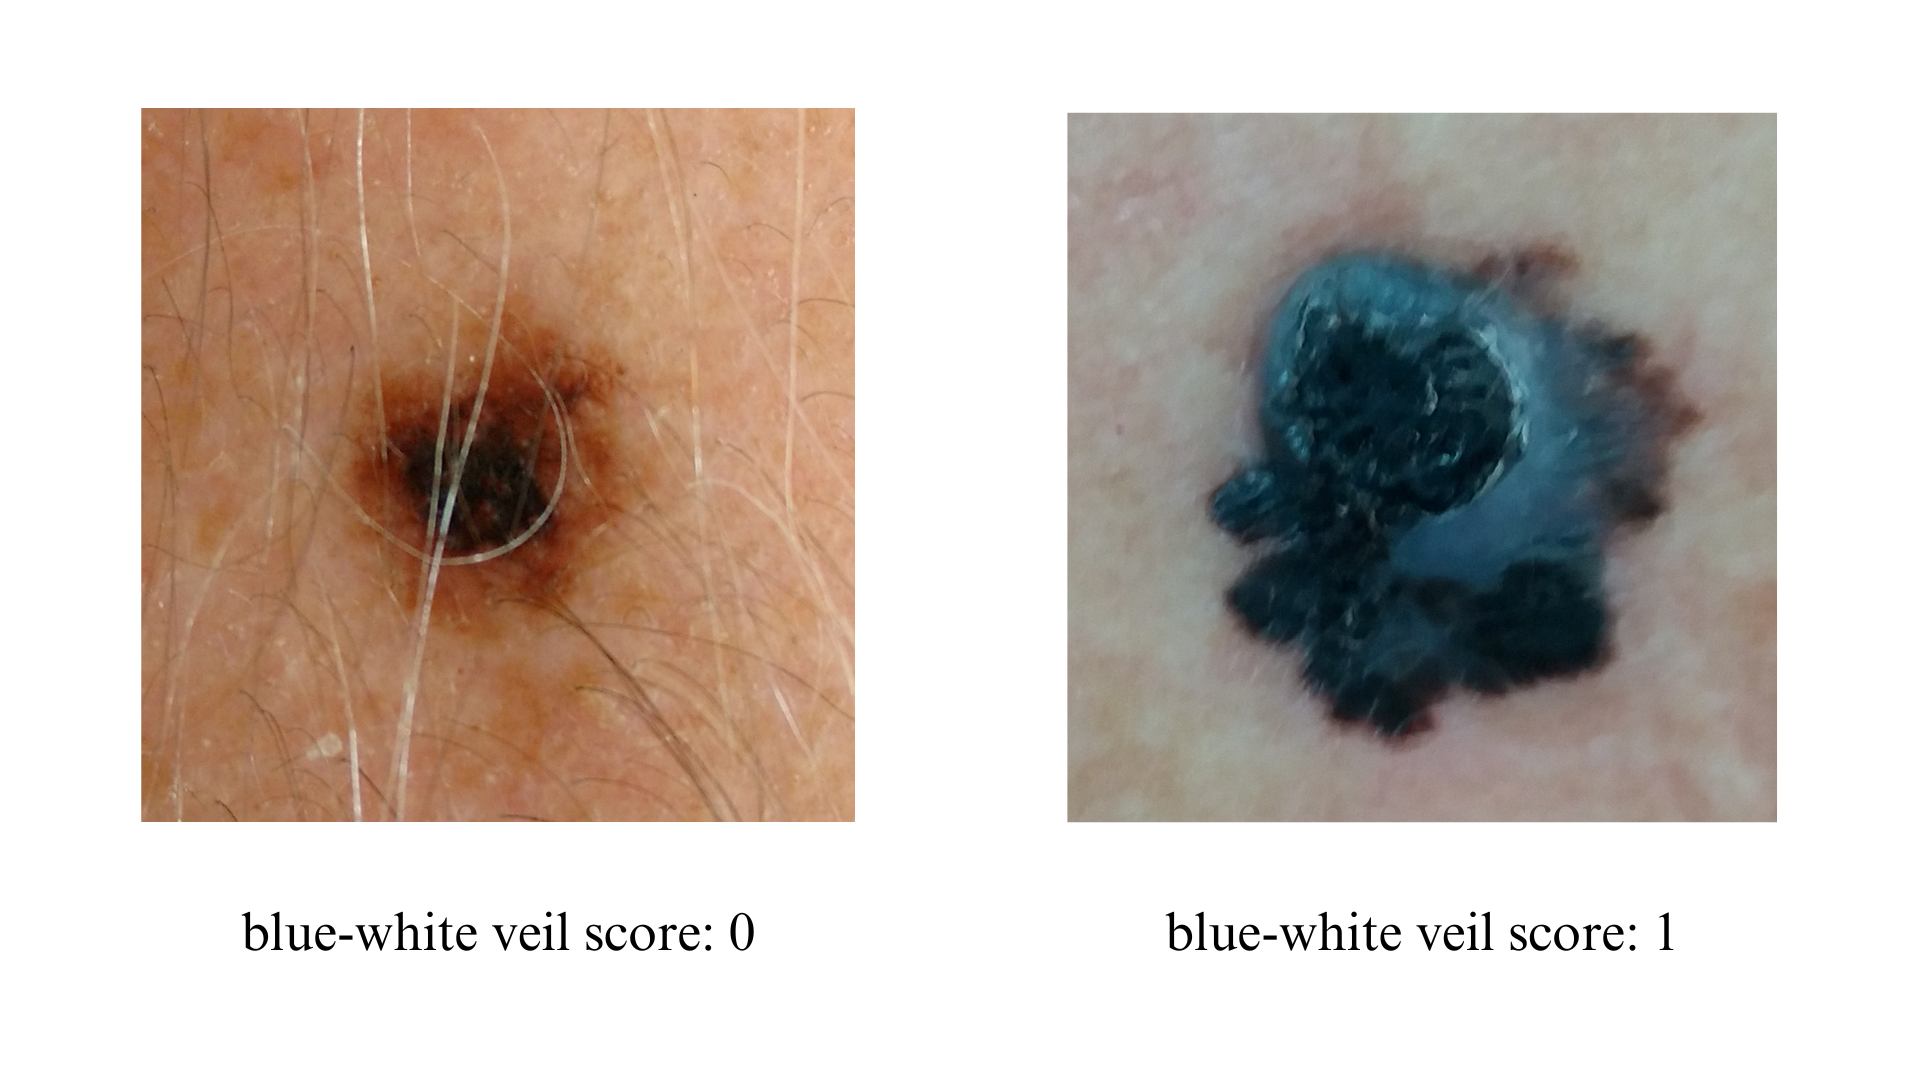
\includegraphics[width=1\linewidth]{blue-white veill.png}
    \caption{Blue-white veil score}
    \label{fig:Blue-white veil score}
\end{figure}

\noindent Based on our manual annotation guide, we gave a score for each of the three features to 120 images (the pictures we created masks for during the first part of the project).
\newline
To apply the scoring system on a larger scale we have written four algorithms to measure the features and segment the lesions.

\subsubsection{Asymmetry}
The algorithm to calculate the asymmetry relies upon a helper function
"FindMajorAxes" which is described below.

\makeatletter
\def\BState{\State\hskip-\ALG@thistlm}
\makeatother
\begin{algorithm}[H]
\caption{FindMajorAxes}
\begin{algorithmic}[1]
\Procedure{FindMajorAxes}{}
\State $major\_axes\_max \gets \text{None}$
\State $mask\_max \gets \text{None}$
\BState \textbf{loop:}
\For{$\text{angle} \gets 0 \text{ to } 180 \text{ by } 10$}
    \State $mask \gets \text{rotate(mask, angle)}$
    \If{$\text{major axes} > major\_axes\_max$}:
        \State $major\_axes\_max \gets \text{major axes}$
        \State $mask\_max \gets \text{mask}$
    \EndIf
\EndFor
\BState \textbf{return} $major\_axes\_max, mask\_max$
\EndProcedure
\end{algorithmic}
\end{algorithm}

\noindent As it can be seen the algorithm rotates a given mask and looks for the largest two axes it can find, compares it to the current largest and updates accordingly. Once the major axes have been found along with the rotation of the mask, the asymmetry index is calculated. The image is folded along the major axes and the overlap is computed to calculate the asymmetry-index.

\[
\text{Asymmetry\_index} = \frac{2 \times |A \cap B|}{|A| + |B|}
\]
where:
\begin{align*}
A & : \text{Overlap along 1st axis} \\
B & : \text{Overlap along 2nd axis} \\
|A| & : \text{Total area lesion} A \\
|B| & : \text{Total area lesion} B \\
|A \cap B| & : \text{Area of the intersection of } A \text{ and } B
\end{align*}

\subsubsection{Colour}
To get a value for the colour variation we are going through the following steps:
\begin{enumerate}
    \item Crop the original image to the size of the lesion in the provided mask:\\
    As we are only interested in the colour variation within the lesion we don't want outside information to influence the rating.
    \item Segment the image into larger "superpixels" and average out the colour:\\
    This is performed by the SLIC ("Simple Linear Iterative Clustering") algorithm, which method uses k-means clustering to create segments with roughly the same colour within the marked area. We average out the colours of these segments to get a uniform value within these.
    \item Convert the image to gray-scale:\\
    We convert the averaged out result to gray-scale to get a single numerical value per segment, we then compare against the other segments. If the values are far apart we can deduct that there are different intensities in the image and thus a higher colour variation and vice versa.
    \item Plot the values to a histogram:\\
    A histogram of such an image represents the distribution of these intensity values. To account for natural variation in the values we summarize the values into a histogram with 30 bins. Given that the colour intensity can vary between 0 and 255 we therefore have a range of 8.5 per column. To filter out any potential noise - e.g. a mask that slightly included also a non lesion part of the image - we take a 95\% interval of the values.
    The values we take from the histogram are the amount of columns that appear in the image, as well as the span between the first and the last column.
\end{enumerate}
The number of columns in the histogram signifies the number of distinct intensity levels present in the image. A larger number of columns implies a greater range of intensities, suggesting more nuanced variations in brightness. A histogram with a broad distribution of columns and diverse spans suggests high colour variation in the image. Conversely, a narrow histogram with clustered columns and limited spans implies a more uniform distribution of intensity values, indicating less variation. 

\begin{figure}[H]
    \centering
    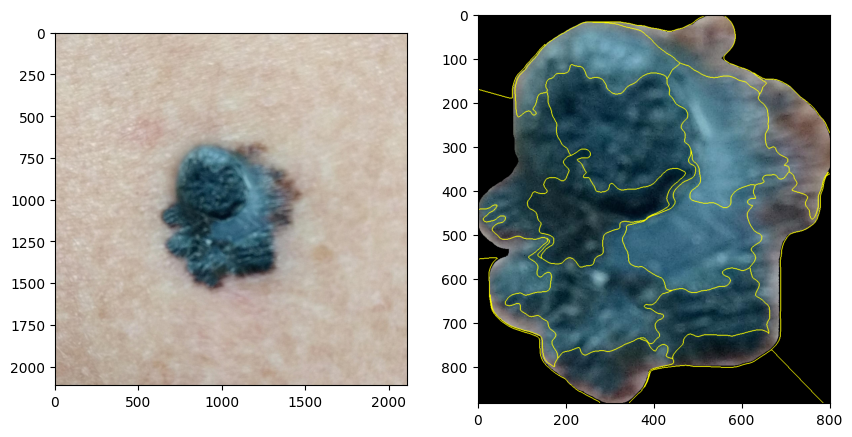
\includegraphics[width=1\linewidth]{Original_Segmentation.png}
    \caption{Original and visualized SLIC segmentations}
    \label{fig:enter-label}
\end{figure}
\begin{figure}[H]
    \centering
    \includegraphics[width=1\linewidth]{Averagecolor_GrayScale.png}
    \caption{Averaged colours and gray-scale}
    \label{fig:enter-label}
\end{figure}

\subsubsection{Blue-White Veil}
In our project, we focused on the detection of blue-white veil in skin lesions, as the extra feature from the 7-point checklist \cite{seven-pointchecklist}.
\newline
The algorithm is designed to process a picture with its corresponding mask. The mask is applied to the image to isolate the lesion, with the rest of the picture set to black.
\newline
After that, we use the SLIC function to segment the lesion based on colour similarity. We get multiple segments of the skin lesion, for each of them we calculate the average RGB values and compare the result to a specific and predefined range of RGB values for blue-white veil. We set this range based on several experiments, especially focused on melanoma pictures, to be in alignment with our expectations on what a blue-white veil should be. If the average colour of a segment is in this range, its area is added to the area of segments containing this feature.
\newline
The final step of the algorithm involves calculating the proportion of the skin lesion affected by blue-white veil by dividing the area of blue-white veil segments with the total area of the lesion. If the value of this proportion is between 20\% and 80\% of the total lesion, it is classified as containing blue-white veil giving a score of 1, and 0 otherwise. We use this criterion in order to guarantee a balanced approach since blue-white veil should cover a significant part of the skin lesion, however not all of it \cite{seven-pointchecklist}.\\
So, the range to determine if a given skin lesion is affected by blue-white veil is: \[20\%\le\frac{\text{area of skin lesion containing blue-white veil}}{\text{total area of skin lesion}}\le80\%\]
\newpage
\noindent The pseudo-code for detecting blue-white veil is the following:

\begin{algorithm}[H]
\caption{Blue-White Veil}
\begin{algorithmic}[1]
\Procedure{Blue-White Veil}{}
\State $segments \gets \text{SLIC}(lesion)$
\State $Area\_bw \gets 0$
\BState \textbf{loop:}
\For{each $segment$ in $segments$}
    \If{$\text{avg\_colour}(segment) \in \text{range\_bw}$}
        \State $Area\_bw \gets Area\_bw + segment$
    \EndIf
\EndFor
\If{$0.2 \leq Proportion\_bw \leq 0.8$}
    \State \Return 1
\Else
    \State \Return 0
\EndIf
\end{algorithmic}
\end{algorithm}

\subsubsection{Segmentation}
In our project, we experimented with three distinct colour-based thresholding methods for segmentation: Otsu's method, mean thresholding, and manual value thresholding. These techniques were selected to outline objects from backgrounds based on intensity levels. However, we encountered inconsistent and unreliable results, particularly when dealing with images featuring varied lighting conditions or complex backgrounds. Additionally, we explored shape-based segmentation techniques, but found their results to be even more inconsistent and less reliable. Consequently, we opted to incorporate manual masks for segmentation, enabling precise definition of objects based on both colour and shape cues. This approach was chosen to enhance the segmentation accuracy and robustness, addressing the limitations observed with solely colour-based methods, especially since the rest of the code in the feature extraction process heavily relied on the masks' quality.

\begin{figure}[H]
    \centering
    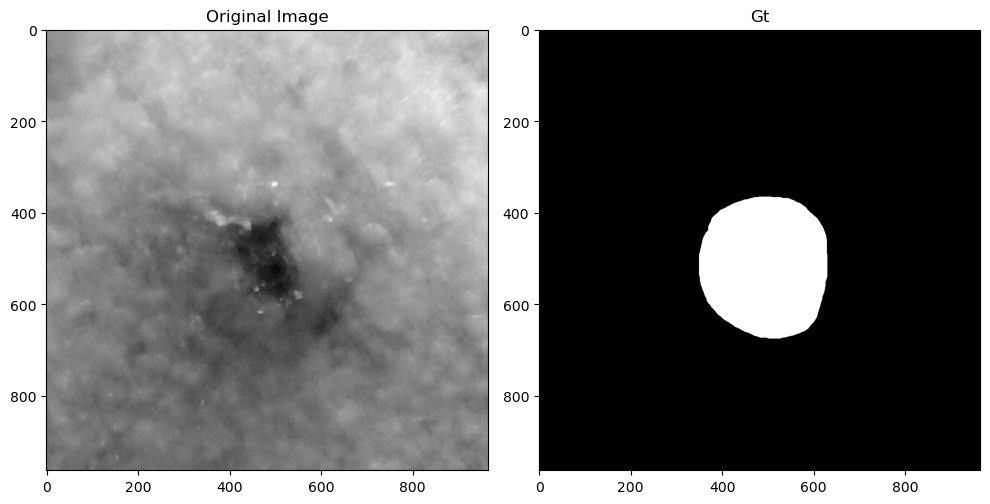
\includegraphics[width=1\linewidth]{original_gt.png}
    \caption{Original image and manual mask}
    \label{fig:enter-label}
\end{figure}
\begin{figure}[H]
    \centering
    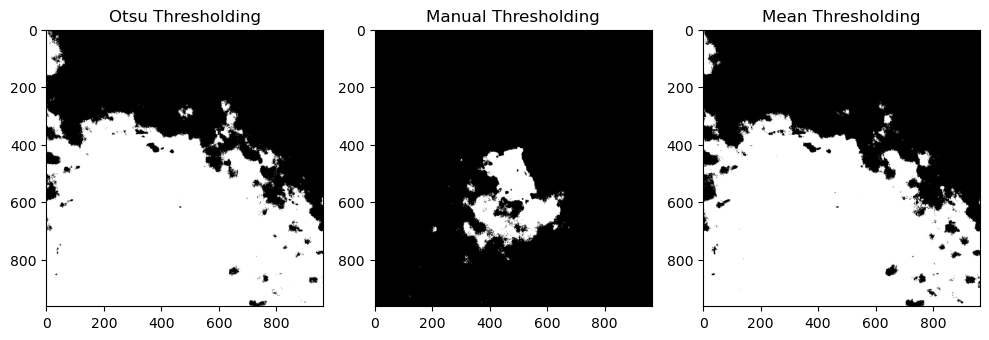
\includegraphics[width=1\linewidth]{result_segmentation.png}
    \caption{Results of automated masking}
    \label{fig:enter-label}
\end{figure}